\documentclass[a4paper, 10pt]{extarticle}

\usepackage[utf8]{inputenc}
\usepackage[russian]{babel}
\usepackage[paper=a4paper, left=15mm, right=15mm, top=0mm, bottom=0mm]{geometry}
\usepackage{graphicx}
\usepackage{xcolor}
\usepackage{transparent}
\usepackage{changepage}
\usepackage{enumitem}
\usepackage{libertine}
\usepackage{fancyhdr}
\usepackage{paracol}
\usepackage[
    colorlinks=true,
    linkcolor=blue,
    citecolor=green,
    filecolor=magenta,
    urlcolor=blue
]{hyperref}

\linespread{1}
\setlength{\parindent}{1.25cm}
\setlength{\parskip}{1em}

\definecolor{blue}{HTML}{074799}

\columnratio{0.35,0.65}
\setlength{\columnsep}{40pt}

\newcommand{\ContactInfo}{
    \hspace{20.5em}\textbf{КОНТАКТНАЯ ИНФОРМАЦИЯ}

    \noindent\hspace{20.5em}Телефон: +7-967-281-53-04
    \hspace{2em}Почта: trud2004@yandex.ru
    \vspace{-1em}
    
    \noindent\hspace{20.5em}Телеграмм: \href{https://t.me/Nep_pasha}{@Nep\_pasha}
    \noindent\hspace{2.5em}Github: \href{https://github.com/nepavellab}{@nepavellab}
}

\newcommand{\Hat}{
\begin{adjustwidth}{-15mm}{-15mm}
    \colorbox{blue}{
        \begin{minipage}[b][140pt][c]{\linewidth}
            \hspace{1.3cm}\parbox{0.1\textwidth}{
                \vspace{7em}
                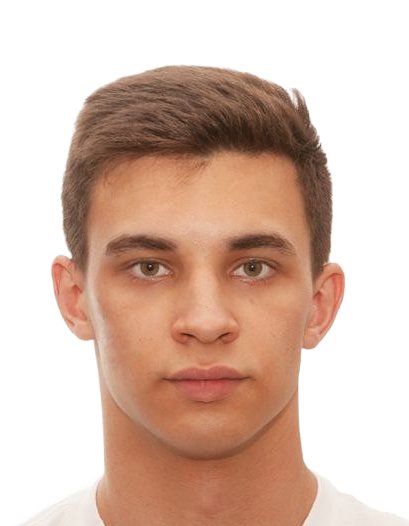
\includegraphics[width=0.275\columnwidth, height=0.35\textwidth]{img/profile.png}
            }
            \parbox{0.9\textwidth}{
                \begin{center}
                    \textcolor{white}{\huge{\transparent{0.8}{Android разработчик}}}
                    \vspace{1em}

                    \textcolor{white}{\Huge{\textbf{НЕПОМНЯЩИХ \\ПАВЕЛ}}}
                \end{center}
            }
        \end{minipage}
    }
\end{adjustwidth}
\ContactInfo
}

\begin{document}
    \Hat

    \begin{paracol}{2}
        \switchcolumn[0]
        \begin{leftcolumn}
            \noindent\rule{\columnwidth}{2pt}
            
            \noindent\textbf{ТЕХНИЧЕСКИЕ НАВЫКИ}
            \begin{itemize}[label=\textcolor{blue}{\textbullet}, topsep=0cm, leftmargin=0.275cm]
                \item Знание базовых алгоритмов \\и структур данных
                \item Опыт работы с параллельностью, \\многопоточностью и\\ асинхронностью
                \item Понимание архитектур\\ MVC, MVP и MVVM
                \item Опыт работы с реляционными и\\ нереляционными базами данных
                \item Навыки с командной строкой и системами контроля версий
            \end{itemize}

            \noindent\rule{\columnwidth}{2pt}
            
            \noindent\textbf{СТЕК ТЕХНОЛОГИЙ}
            \begin{itemize}[
                label=\textcolor{blue}{\textbullet}, 
                topsep=0cm,
                leftmargin=0.275cm,
                itemsep=0.1cm
            ]
                \item Языки программирования: \\C/C++, Java, Kotlin, Python
                \item SQL (SQLite, PostgreSQL), Firebase
                \item Andorid Framework
                \item Jetpack Compose
                \item Библотеки: Room, Retrofit, Dagger 2
            \end{itemize}
        \end{leftcolumn}

        \switchcolumn[1]
        \begin{rightcolumn}
            \noindent\rule{\columnwidth}{2pt}
            
            \noindent\textbf{ОБРАЗОВАНИЕ}
            \vspace{1em}

            \noindent\parbox{0.1\columnwidth}{
                
\includegraphics[width=0.05\textwidth]{img/bmstu_logo.png}
            }
            \parbox{0.85\columnwidth}{
                \textbf{МГТУ им. Н.Э. Баумана}
                \hfill \textbf{Москва}
                \vspace{0.5em}
                \hrule
                \vspace{0.5em}

                Направление: \hfill \textit{2022 -- н.в.} 
                
                \textit{Математика и компьютерные науки}
            }

            \noindent\rule{\columnwidth}{2pt}

            \noindent\textbf{ДОПОЛНИТЕЛЬНОЕ ОБРАЗОВАНИЕ}

            \noindent\parbox{0.1\columnwidth}{
                
\includegraphics[width=0.05\textwidth]{img/tbank_logo.png}
            }
            \parbox{0.85\columnwidth}{
                \textbf{Курс Т-Банк \& МГТУ им. Н.Э. Баумана}
                \hfill \textbf{Москва}
                \hrule
                \vspace{0.5em}

                Программа: \textit{Android разработчик}
                \hfill \textit{2022 -- 2022} 
            }
            \vspace{1em}

            \noindent\parbox{0.1\columnwidth}{
                
\includegraphics[width=0.05\textwidth]{img/vk_logo.png}
            }
            \parbox{0.85\columnwidth}{
                \textbf{<<Технопарк>> (VK \& МГТУ им. Н. Э. Баумана)}
                \hfill \textbf{Москва}
                \hrule
                \vspace{0.5em}

                Программа: \textit{Android разработчик}
                \hfill \textit{2022 -- н.в.} 
            }
        \end{rightcolumn}
    \end{paracol}
\end{document}